% ============================================================
%  Fig_counterfactual_cycle.tex
%  因果推論：反実仮想によるビジネスサイクルと政策効果
%  「政策なしなら、もっと悪化していた」を示すtime-series図
%  upLaTeX + dvipdfmx / standalone
% ============================================================
\documentclass[tikz, dvipdfmx]{standalone}
\usepackage{tikz}
\usetikzlibrary{arrows.meta, decorations.pathreplacing, calligraphy}

% ── 色定義（Fig_causal_simple.tex と統一） ──────────────────
\definecolor{gdpblue}{RGB}{30,  90, 180}   % 観測軌跡
\definecolor{obscol} {RGB}{210, 228, 255}  % 観測可能（薄青）
\definecolor{cfcol}  {RGB}{232, 232, 232}  % 観測不可（薄灰）
\definecolor{fillcol}{RGB}{180, 215, 255}  % 政策効果の差分領域

\begin{document}
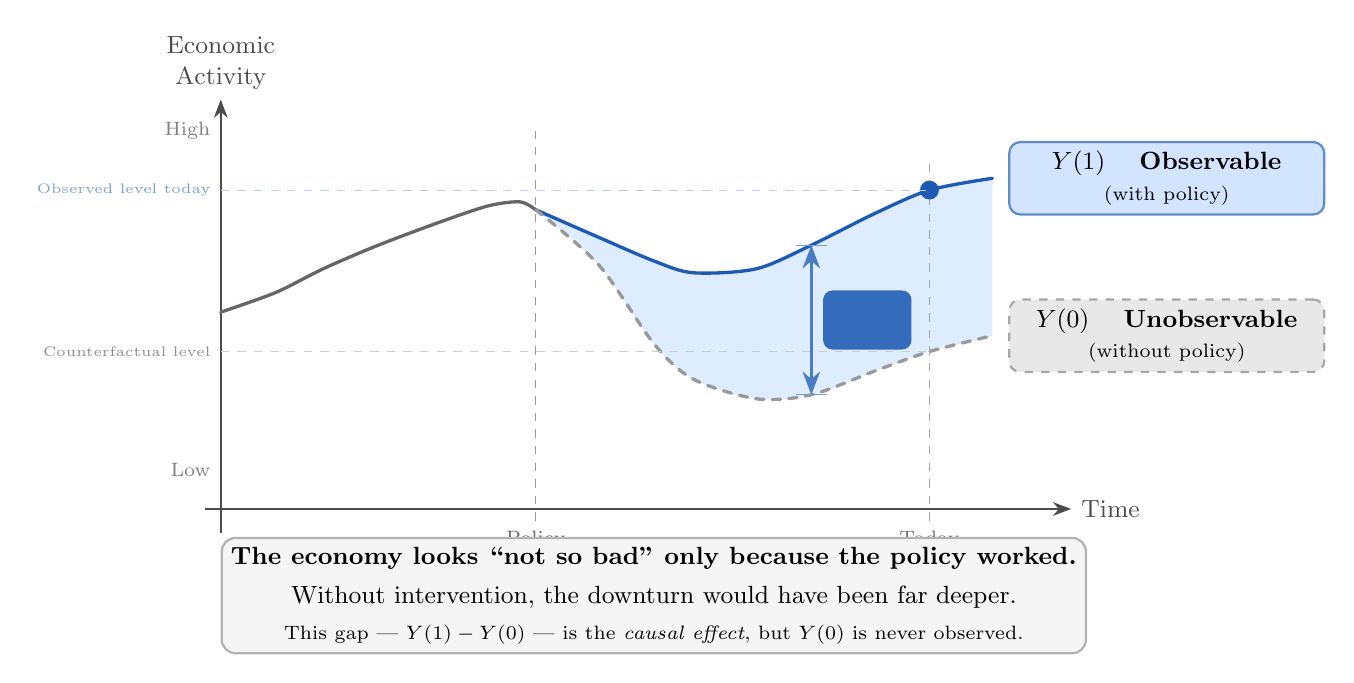
\begin{tikzpicture}[
  >=Stealth,
  thick,
  every node/.style={font=\small},
  % 単位: 1 = 1cm
]

% ============================================================
%  0.  差分領域（一番先に描いてから線を上書き）
% ============================================================
\fill[fillcol, opacity=0.45]
  % 観測軌跡（政策あり）：前進方向
  plot[smooth, tension=0.5] coordinates {
    (4.0, 3.80)
    (4.8, 3.45)
    (5.5, 3.15)
    (6.0, 3.00)
    (6.8, 3.05)
    (7.5, 3.35)
    (8.3, 3.75)
    (9.0, 4.05)
    (9.8, 4.20)
  }
  % 反実仮想（政策なし）：逆順でパスを閉じる
  -- plot[smooth, tension=0.5] coordinates {
    (9.8, 2.20)
    (9.0, 2.00)
    (8.3, 1.75)
    (7.5, 1.45)
    (6.8, 1.40)
    (6.0, 1.65)
    (5.5, 2.10)
    (4.8, 3.10)
    (4.0, 3.80)
  } -- cycle;

% ============================================================
%  1.  座標軸
% ============================================================
% 横軸
\draw[->, thick, black!70]
  (-0.2, 0) -- (10.8, 0)
  node[right, font=\small] {Time};

% 縦軸
\draw[->, thick, black!70]
  (0, -0.3) -- (0, 5.2)
  node[above, font=\small, align=center] {Economic\\Activity};

% 縦軸の High / Low ラベル
\node[font=\scriptsize, black!50, left] at (0, 4.8) {High};
\node[font=\scriptsize, black!50, left] at (0, 0.5) {Low};

% ============================================================
%  2.  政策前の共通軌跡（t = 0 → 4）
%      緩やかな成長からピーク、危機の予兆へ
% ============================================================
\draw[black!60, very thick, line cap=round]
  plot[smooth, tension=0.5] coordinates {
    (0.0, 2.50)
    (0.7, 2.75)
    (1.3, 3.05)
    (2.0, 3.35)
    (2.8, 3.65)
    (3.4, 3.85)
    (3.8, 3.90)
    (4.0, 3.80)
  };

% ============================================================
%  3.  政策介入点（t = 4）の縦線
% ============================================================
\draw[dashed, black!40, thin]
  (4.0, -0.15) -- (4.0, 4.80);

\node[font=\scriptsize, black!60, align=center, below]
  at (4.0, -0.15)
  {Policy\\Intervention};

% ============================================================
%  4.  観測軌跡（政策あり、t = 4 → 9.8）  実線・青
% ============================================================
\draw[gdpblue, very thick, line cap=round]
  plot[smooth, tension=0.5] coordinates {
    (4.0, 3.80)
    (4.8, 3.45)
    (5.5, 3.15)
    (6.0, 3.00)
    (6.8, 3.05)
    (7.5, 3.35)
    (8.3, 3.75)
    (9.0, 4.05)
    (9.8, 4.20)
  };

% 観測軌跡ラベルボックス
\node[
  draw=gdpblue!70, fill=obscol,
  rounded corners=4pt,
  minimum width=4.0cm, minimum height=0.9cm,
  align=center, anchor=west, font=\small,
] (obs_box) at (10.0, 4.20)
  {$Y(1)$ \quad \textbf{Observable}\\
   {\scriptsize (with policy)}};

% ============================================================
%  5.  反実仮想（政策なし、t = 4 → 9.8）  破線・グレー
% ============================================================
\draw[black!40, very thick, dashed, line cap=round]
  plot[smooth, tension=0.5] coordinates {
    (4.0, 3.80)
    (4.8, 3.10)
    (5.5, 2.10)
    (6.0, 1.65)
    (6.8, 1.40)
    (7.5, 1.45)
    (8.3, 1.75)
    (9.0, 2.00)
    (9.8, 2.20)
  };

% 反実仮想ラベルボックス
\node[
  draw=black!35, fill=cfcol,
  dashed, rounded corners=4pt,
  minimum width=4.0cm, minimum height=0.9cm,
  align=center, anchor=west, font=\small,
] (cf_box) at (10.0, 2.20)
  {$Y(0)$ \quad \textbf{Unobservable}\\
   {\scriptsize (without policy)}};

% ============================================================
%  6.  "Today" マーカー（t = 9）
% ============================================================
\draw[dashed, black!35, thin]
  (9.0, -0.15) -- (9.0, 4.40);

\node[font=\scriptsize, black!55, below]
  at (9.0, -0.15) {Today};

% 観測点（Today）のドット
\filldraw[gdpblue] (9.0, 4.05) circle (3pt);

% ============================================================
%  7.  Policy Effect の双方向矢印（t ≈ 7.5）
% ============================================================
% 矢印
\draw[<->, very thick, gdpblue!80]
  (7.5, 1.45) -- (7.5, 3.35);

% ラベル
\node[
  fill=white, draw=gdpblue!40,
  rounded corners=3pt,
  font=\scriptsize, gdpblue!90,
  align=center, anchor=west,
] at (7.65, 2.40)
  {\textbf{Policy}\\[1pt]\textbf{Effect}};

% 上端・下端の水平ティック
\draw[gdpblue!60, thin] (7.3, 3.35) -- (7.7, 3.35);
\draw[gdpblue!60, thin] (7.3, 1.45) -- (7.7, 1.45);

% ============================================================
%  8.  「現在の観測値」水平参照線（薄い）
% ============================================================
\draw[gdpblue!30, thin, dashed]
  (0.0, 4.05) -- (9.0, 4.05);
\node[font=\tiny, gdpblue!60, left] at (0.0, 4.05)
  {Observed level today};

\draw[black!20, thin, dashed]
  (0.0, 2.00) -- (9.0, 2.00);
\node[font=\tiny, black!45, left] at (0.0, 2.00)
  {Counterfactual level};

% ============================================================
%  9.  下部メッセージボックス
% ============================================================
\node[
  draw=black!30, fill=black!4,
  rounded corners=5pt,
  font=\small, align=center,
  minimum width=9.5cm,
] at (5.5, -1.1)
  {\textbf{The economy looks ``not so bad'' only because the policy worked.}\\[3pt]
   {\small Without intervention, the downturn would have been far deeper.}\\[2pt]
   {\scriptsize This gap — $Y(1) - Y(0)$ — is the \emph{causal effect}, but $Y(0)$ is never observed.}};

\end{tikzpicture}
\end{document}
